%https://www.sharelatex.com/learn/Typesetting_quotations
%https://tex.stackexchange.com/questions/69997/how-to-write-an-m%E2%A8%89n-matrix-in-latex
%https://tex.stackexchange.com/questions/119319/how-to-correctly-shrink-the-bullets-of-itemize
\documentclass[titlepage,a4paper]{article}
\usepackage{graphicx}
\usepackage{tikz-qtree}
\usepackage{amsmath}
\usepackage{csquotes}
\renewcommand\labelitemi{$\bullet$}
\renewcommand\descriptionlabel{$\cdot$}
\begin{document}

\title{ \textbf{SSL Inlab \\ Advanced \LaTeX} }
\author{ \huge{Contour} \\ \large{160050002} \\  \large{160050056} \\ \large{160050057} }
\date{24 August}
\maketitle

\tableofcontents

\newpage

\section{Itemize, Enumerate and Description}
\subsection{Itemize}
	\begin{itemize}
		\item \LaTeX typesets a file of text using the TEX program.
		\item \LaTeX is widely used in academia for the communication and publication
of scientific documents in many fields, including mathematics, physics,
computer science, statistics, economics and political science.
		\item \LaTeX can be used as a standalone document preparation system or as an
intermediate format.
		\item \textbf{Have used renewcommand for the bullets to be bigger.}
	\end{itemize}
\subsection{Enumerate}
	\begin{enumerate}
		\item \LaTeX typesets a file of text using the TEX program.
		\item \LaTeX is widely used in academia for the communication and publication
of scientific documents in many fields, including mathematics, physics,
computer science, statistics, economics and political science.
		\item \LaTeX can be used as a standalone document preparation system or as an
intermediate format.
		\item \LaTeX is intended to provide a high-level language that accesses the power
of TeX in an easier way for writers.
	\end{enumerate}

\subsection{Description}
	\begin{description}
		\item[\textbf{Red}] A colour at the end of the spectrum next to orange and opposite violet,
as of blood, fire, or rubies. program.
		\item[\textbf{Blue}] A colour intermediate between green and violet, as of the sky or sea on
a sunny day.
		\item[\textbf{White}] The colour of milk or fresh snow, due to the reflection of all visible
rays of light; the opposite of black.
		\item[\textbf{Black}] The darkest colour owing to the absence of or complete absorption of
light; the opposite of white.
	\end{description}

\section{Mathematical formulas and notations}
\subsection{Matrix}
\begin{tabular}{c|c}
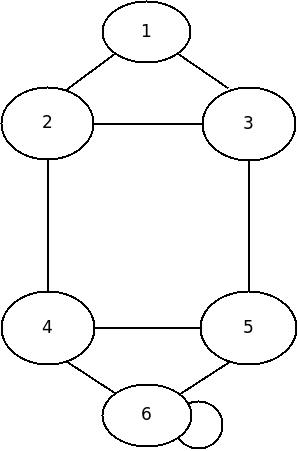
\includegraphics[width=0.5\textwidth]{diagramSection2.jpeg}
&
\bordermatrix{ & \textbf{1} & \textbf{2} & \textbf{3} & \textbf{4} & \textbf{5} &
\textbf{6} \cr
        \textbf{1} & 1 & 1 & 1 & 1 & 1 & 1 \cr
        \textbf{2} & 1 & 1 & 1 & 1 & 1 & 1 \cr
        \textbf{3} & 1 & 1 & 1 & 1 & 1 & 1 \cr
        \textbf{4} & 1 & 1 & 1 & 1 & 1 & 1 \cr
        \textbf{5} & 1 & 1 & 1 & 1 & 1 & 1 \cr
        \textbf{6} & 1 & 1 & 1 & 1 & 1 & 1 \cr} \qquad
\end{tabular}

\subsection{Equation Array}
\begin{eqnarray}
cos2\theta & = cos^{2}\theta-sin^{2}\theta\\
&= 2cos^{2}\theta-1
\end{eqnarray}


\subsection{Prepositional Formulae using Various Operators}
$\neg(\forall x)(\varphi(x))\longleftrightarrow(\exists x)\neg\varphi(x)$\\
\\
$(\forall x)(\psi(x)\wedge\psi(x))\longleftrightarrow((\forall x)\varphi(x)\wedge(\forall x)\varphi(x))$
\begin{table}
\begin{tabular}{|c|c|}[h!]
Greek Letters & $\alpha A\ \beta B\ \gamma\Gamma\ \rho\varrho P\ \sigma\Sigma\ \delta\Delta\ \epsilon\varepsilon E$\\
\end{tabular}
\end{table}
\subsection{Mathematical Formulas}
\begin{enumerate}
\item $\frac{\pi}{4}=\sum \limits_{n=0}^{\infty}\frac{(-1)^{n}*\overbrace{(1+1+\cdots+1)}^{n}}{(2n+1)*n}$
\end{enumerate}




\section{Quote}
\subsection{Quote}
The margins of the quote environment are indented on both the left and the
right. The text is justified at both margins. Leaving a blank line between text
produces a new paragraph.The package csquotes offers a multilingual solution
to quotations, with integration to citation mechanisms offered by BibTeX.
\begin{displayquote}
"Unlike the quotation environment, paragraphs are not indented. It’s
important to remark that even if you are typing quotes on English
there are different quotation marks used in English (UK) and English
(US)."
\end{displayquote}

\section{Algorithm and Pseudo code}
\subsection{Tabbing}
\begin{tabbing}
\hspace*{3em}\=\hspace*{3em}\=\hspace*{3em}\=\hspace*{3em}\=\kill
//Breadth First Search Function\\
void BFS(list\textless long long int\textgreater queue,long long int length)\{ \\
\> long long int v; \\
\> if(queue.empty())  \\
\> \>return; \\
\> list long long int ::iterator i; \\
\> list long long int  queue temp; \\
\> while(!queue.empty())\{ \\
\> \> v=queue.front(); \\
\> \> queue.pop front(); \\
\> \> for(i=adj[v].begin();i!=adj[v].end();i++)\{ \\
\> \> \>                if(!pro  ver[*i])\{ \\
\> \> \> \> result[*i]=length; \\
\> \> \> \>                                queue temp.push back(*i); \\
\> \> \> \>                        pro ver[*i]=true; \\
\> \> \> \>                        adj[*i].remove(v); \\
\> \> \>                \} \\
\> \>        \} \\
\>        \}\\
\>BFS(queue temp,length+6);\\
\}
\end{tabbing}

\section{Tree}
\Tree[.If-statement [.If ]
[.exp ]
[.\textit{then} ]
[.S [.if  [.if ]
[.exp ]
[.\textit{then} ]
[.S ]]]]

\end{document}